% !TEX root = ../script.tex
\section{Объективное априорное распределение}

Другим популярным подходом к выбору априорного распределения 
--- помимо прагматичного способа, описанного ранее --- является объективный подход.
В этом подходе наша цель --- выбрать априорное распределение,
которое бы больше всего соответствовало отсутствия каких-либо априорных знаний, неинформативное априорное распределение.
Рассмотрим два естественных примера такого распределения.
% Как мы увидели в разделе~\ref{sec:objective_intro} равномерное априорное распределение не годится, так как при использовании другой параметризации параметров мы получаем уже неравномерное распределение.

\begin{example}[Априорное распределение для параметра сдвига]
Пускай мы хотим выбрать целевое распределение данных из семейства $f(x - \theta)$. 
Естественно предположить, что все параметры сдвига равновероятны --- и мы не можем отдать предпочтение какому-нибудь в нашем неинформативном априорном распределении.

Тогда логично использовать равномерное априорное распределение с плотностью $\pi(\theta) \sim 1$.
Если множество $\Theta$ допустимых значений $\theta$ ограничено, то мы получаем корректное априорное распределение, 
которое соответствует нашим требованиям.

Если множество $\Theta$ неограничено, например, $\Theta = \bbR$, то если мы возьмем плотность $\pi(\theta) \sim 1, \theta \in \Theta$,
которая не будет отвечать никакому вероятностному распределению, так как интеграл $\int_{\Theta} \pi(\theta) d\theta$ не будет конечным.
Такое априорное распределение называется \emph{некорректным априорным распределением}.

Однако, в некоторых случаях некорректное априорное распределение оказывается полезным.
Часто для некорректного априорного распределения апостериорное распределение оказывается корректным.
В частности, подход к выбору $\theta$ на основе максимизации правдподобия соотвествует Байесовскому подходу с равномерным на $\bbR$ 
априорным распределением.

Так же можно определить такое некорректное априорное распределение как предел последовательности корректных априорных распределений.
Тем самым получится математически строго работать с объектами Байесовского статистики.
\end{example}

\begin{example}[Априорное распределение для параметра масштаба]
Введем равномерное распределение для параметра масштаба.
Параметр масштаба --- такой параметр плотности, что для $\theta \in \Theta \subseteq \bbR^+$:
\[
f_\theta(x) = \frac{1}{\theta} f^0 \left(\frac{x}{\theta} \right),
\]
отношение $\frac{1}{\theta}$ здесь нужно для нормализации распределения.
Тогда если мы захотим потребовать от априорного распределения инвариантности к масштабу, 
то для любого $c > 0$ должно быть выполнено, что
\[
\pi(\theta) = \frac{1}{c} \pi \left(\frac{\theta}{c} \right).
\]
У такого функционального уравнения существует единственное с точностью до масштабирующего коэффициента решение:
\[
\pi(\theta) \sim \frac{1}{\theta}.
\]
Отметим, что мы --- как и при выборе априорного распределения для параметра сдвига --- получили некорректное неинформативное распределение для масштаба,
что, на самом деле, часто не является проблемой.

Рассмотрим теперь $\rho = \log \theta$.
Тогда 
\[
\pi(\rho) = \pi(\theta) \left| \frac{d \theta}{d \rho} \right| \sim e^{-\rho} e^{\rho} = 1.
\]
То есть, неинформативное априорное распределение для такого преобразования параметра масштаба будет равномерным.

Можно получить такое априорное распределение и другим способом.
% TODO
\end{example}


% Естественной идеей будет выбрать априорное распределение, которое не будет зависеть от параметризации.
% Такое априорное распределение называется \emph{опорным априорным распределением}.

\subsection{Априорное распределение Джеффриса}

Мы хотели бы работать с априорным распределением, на которое не будет влиять параметризация $\theta$.
Оказывается, такое априорное распределение существует:
\[
\pi_J(\theta) \sim I(\theta)^{\frac12},
\]
где $I(\theta)^{\frac12}$ --- информационная матрица Фишера или информация Фишера \index{информация Фишера}:
\[
I(\theta) = - \bbE_{\theta} \left[\frac{d^2 \log p(x| \theta)}{d \theta^2} \right].
\]
Информационная матрица Фишера --- важный объект в классической математической статистике.
Легко видеть, что она локально вогнута в окрестности оценки максимума правдоподобия 
и глобально вогнута для экспоненциального семейства распределений. % TODO Exercise

Докажем теперь, что априорное распределение Джеффриса не зависит от параметризации.
\begin{proof}

Сперва докажем лемму
\begin{Lemma}
\label{lemma:bbeEqZero}
Если правдоподобие --- регулярно (то есть, можно выносить дифференцирования по параметру за интеграл), то
для математического ожидания производной логарифма правдоподобия по параметру выполнено:
\[
\bbE \left(\frac{d \log p(x | \theta)}{d \theta} \right) = 0.
\]
\end{Lemma}
\begin{proof}
Получаем результат теоремы воспользовавшись регулярностью правдоподобия и условием нормировки для вероятностного распределения $\int p(x| \theta) dx = 1$:
\begin{align*}
\bbE \left(\frac{d \log p(x | \theta)}{d \theta} \right) &= \int \frac{d \log p(x | \theta)}{d \theta} p(x| \theta) dx = \\
                                                         &= \int \frac{d p(x | \theta)}{d \theta} \frac{1}{p(x | \theta)} p(x| \theta) dx =\\
                                                         &= \int \frac{d p(x | \theta)}{d \theta} dx = \frac{d}{d \theta} \int p(x| \theta) dx =\\
                                                         &= \frac{d}{d \theta} 1 = 0. \\
\end{align*}
\end{proof}

Подсчитаем информацию Фишера для другой параметризации $\phi$ параметра $\theta$:
\begin{align*}
I(\phi) &= -\bbE \left[\frac{d^2 \log p(x | \phi)}{d \phi^2} \right] = \\
&= -\bbE \left[\frac{d^2 \log p(x | \theta)}{d \theta^2}  \left(\frac{d \theta}{d \phi} \right)^2 + \frac{d \log p(x | \theta)}{d \theta} \frac{d^2 \theta}{d \phi^2} \right] = \\
&= -\bbE \left[\frac{d^2 \log p(x | \theta)}{d \theta^2}  \left(\frac{d \theta}{d \phi} \right)^2 \right] -\bbE \left[ \frac{d \log p(x | \theta)}{d \theta} \frac{d^2 \theta}{d \phi^2} \right] = \\
&= -\bbE \left[\frac{d^2 \log p(x | \theta)}{d \theta^2} \right] \left(\frac{d \theta}{d \phi} \right)^2.
\end{align*}
При преобразованиях мы воспользовались результатом Леммы~\ref{lemma:bbeEqZero} для того, чтобы избавиться от одного из слагаемых.

Следовательно,
\[
I(\phi) = I(\theta) \left(\frac{d \theta}{d \phi} \right)^2.
\]
Таким образом,
\[
\sqrt{I(\phi)} = \sqrt{I(\theta)} \left| \frac{d \theta}{d \phi} \right|.
\]
Плотность распределения при преобразовании случайной величины имеет вид:
\[
\pi(\phi(\theta)) = \pi(\theta) \left| \frac{d \theta}{d \phi(\theta)} \right|
\]
Получаем:
\[
\pi_J(\theta) = \sqrt{I(\theta)},
\]
что и требовалось доказать.

\end{proof}

\subsection{Примеры априорных распределений Джеффриса}
\begin{example}
Получим априорное распределение Джеффриса для среднего нормального распределения.
Пусть $x \sim \mathcal{N}(\mu, \sigma^2)$, причем $\sigma^2$ известно.
Тогда плотность распределения:
\[
p(x | \mu) \sim \exp \left(- \frac{1}{2 \sigma^2} (x - \mu)^2 \right).
\]
Дифференцируя логарифм правдоподобия два раза получаем:
\[
\frac{d^2 \log p(x | \mu)}{d \mu^2} = -\frac{1}{\sigma^2}.
\]
Таким образом, информация Фишера в таком случае не зависит от $\mu$, и мы получаем равномерное априорное распределение Джеффриса:
\[
\pi_J(\theta) \sim I(\theta)^{\frac12} = \frac{1}{\sigma}.
\]
\end{example}

\begin{example}
Найдем априорное распределение Джеффриса для еще одной широко используемой модели.
Пусть $x \sim \mathrm{Bin}(\sS, \theta)$ --- биномиальная случайная величина с параметрами $\sS$ и $0 \leq \theta \leq 1$.
Тогда правдоподобие для $x \in \mathbb{N} \cup \{0\}$имеет вид:
\[
p(x | \theta) = C_{\sS}^x \theta^x (1- \theta)^{\sS - x}.
\]
Получим априорное распределение Джеффриса:
\[
\log p(x | \theta) \propto x \log \theta + (\sS - x) \log(1 - \theta).
\]
Тогда 
\[
\frac{ d \log p(x | \theta)}{d \theta} \propto \frac{x}{\theta} - \frac{\sS - x}{1 - \theta}.
\]
И
\[
\frac{ d^2 \log p(x | \theta)}{d \theta^2} \propto -\frac{x}{\theta^2} - \frac{\sS - x}{(1 - \theta)^2}.
\]
Для биномиального распределения
\[
\bbE_\theta x = \sS \theta.
\]
Следовательно,
\[
I(\theta) = -\bbE \left[\frac{d^2 \log p(x | \theta)}{d \theta^2} \right] = \frac{n \theta}{\theta^2} + \frac{n - n\theta}{(1 - \theta)^2} =
= \frac{n}{\theta} + \frac{n}{1 - \theta} = \frac{n}{\theta (1 - \theta)}.
\]
Следовательно,
\[
\pi_J(\theta) = \sqrt{I(\theta)} \propto \theta^{-\frac12} (1 - \theta)^{-\frac12}.
\]
Априорное распределение Джеффриса для такой модели $\pi_J(\theta)$ --- бета-распределение с параметрами $\frac12$, $\frac12$.
Данные «меньше всего» влияют на апостериорное распределение, если $\theta = \frac12$, 
и «больше всего», если $\theta = 0$ или $1$.
Использование $\beta(\frac12, \frac12)$ позволяет уравнять эффект добавления данных в модель.
Полезно сравнить это априорное распределение с равномерным распределением $\beta(1, 1)$.
Оба эти распределения приведены на рисунке~\ref{fig:beta_comparison}.

\begin{figure}
\centering
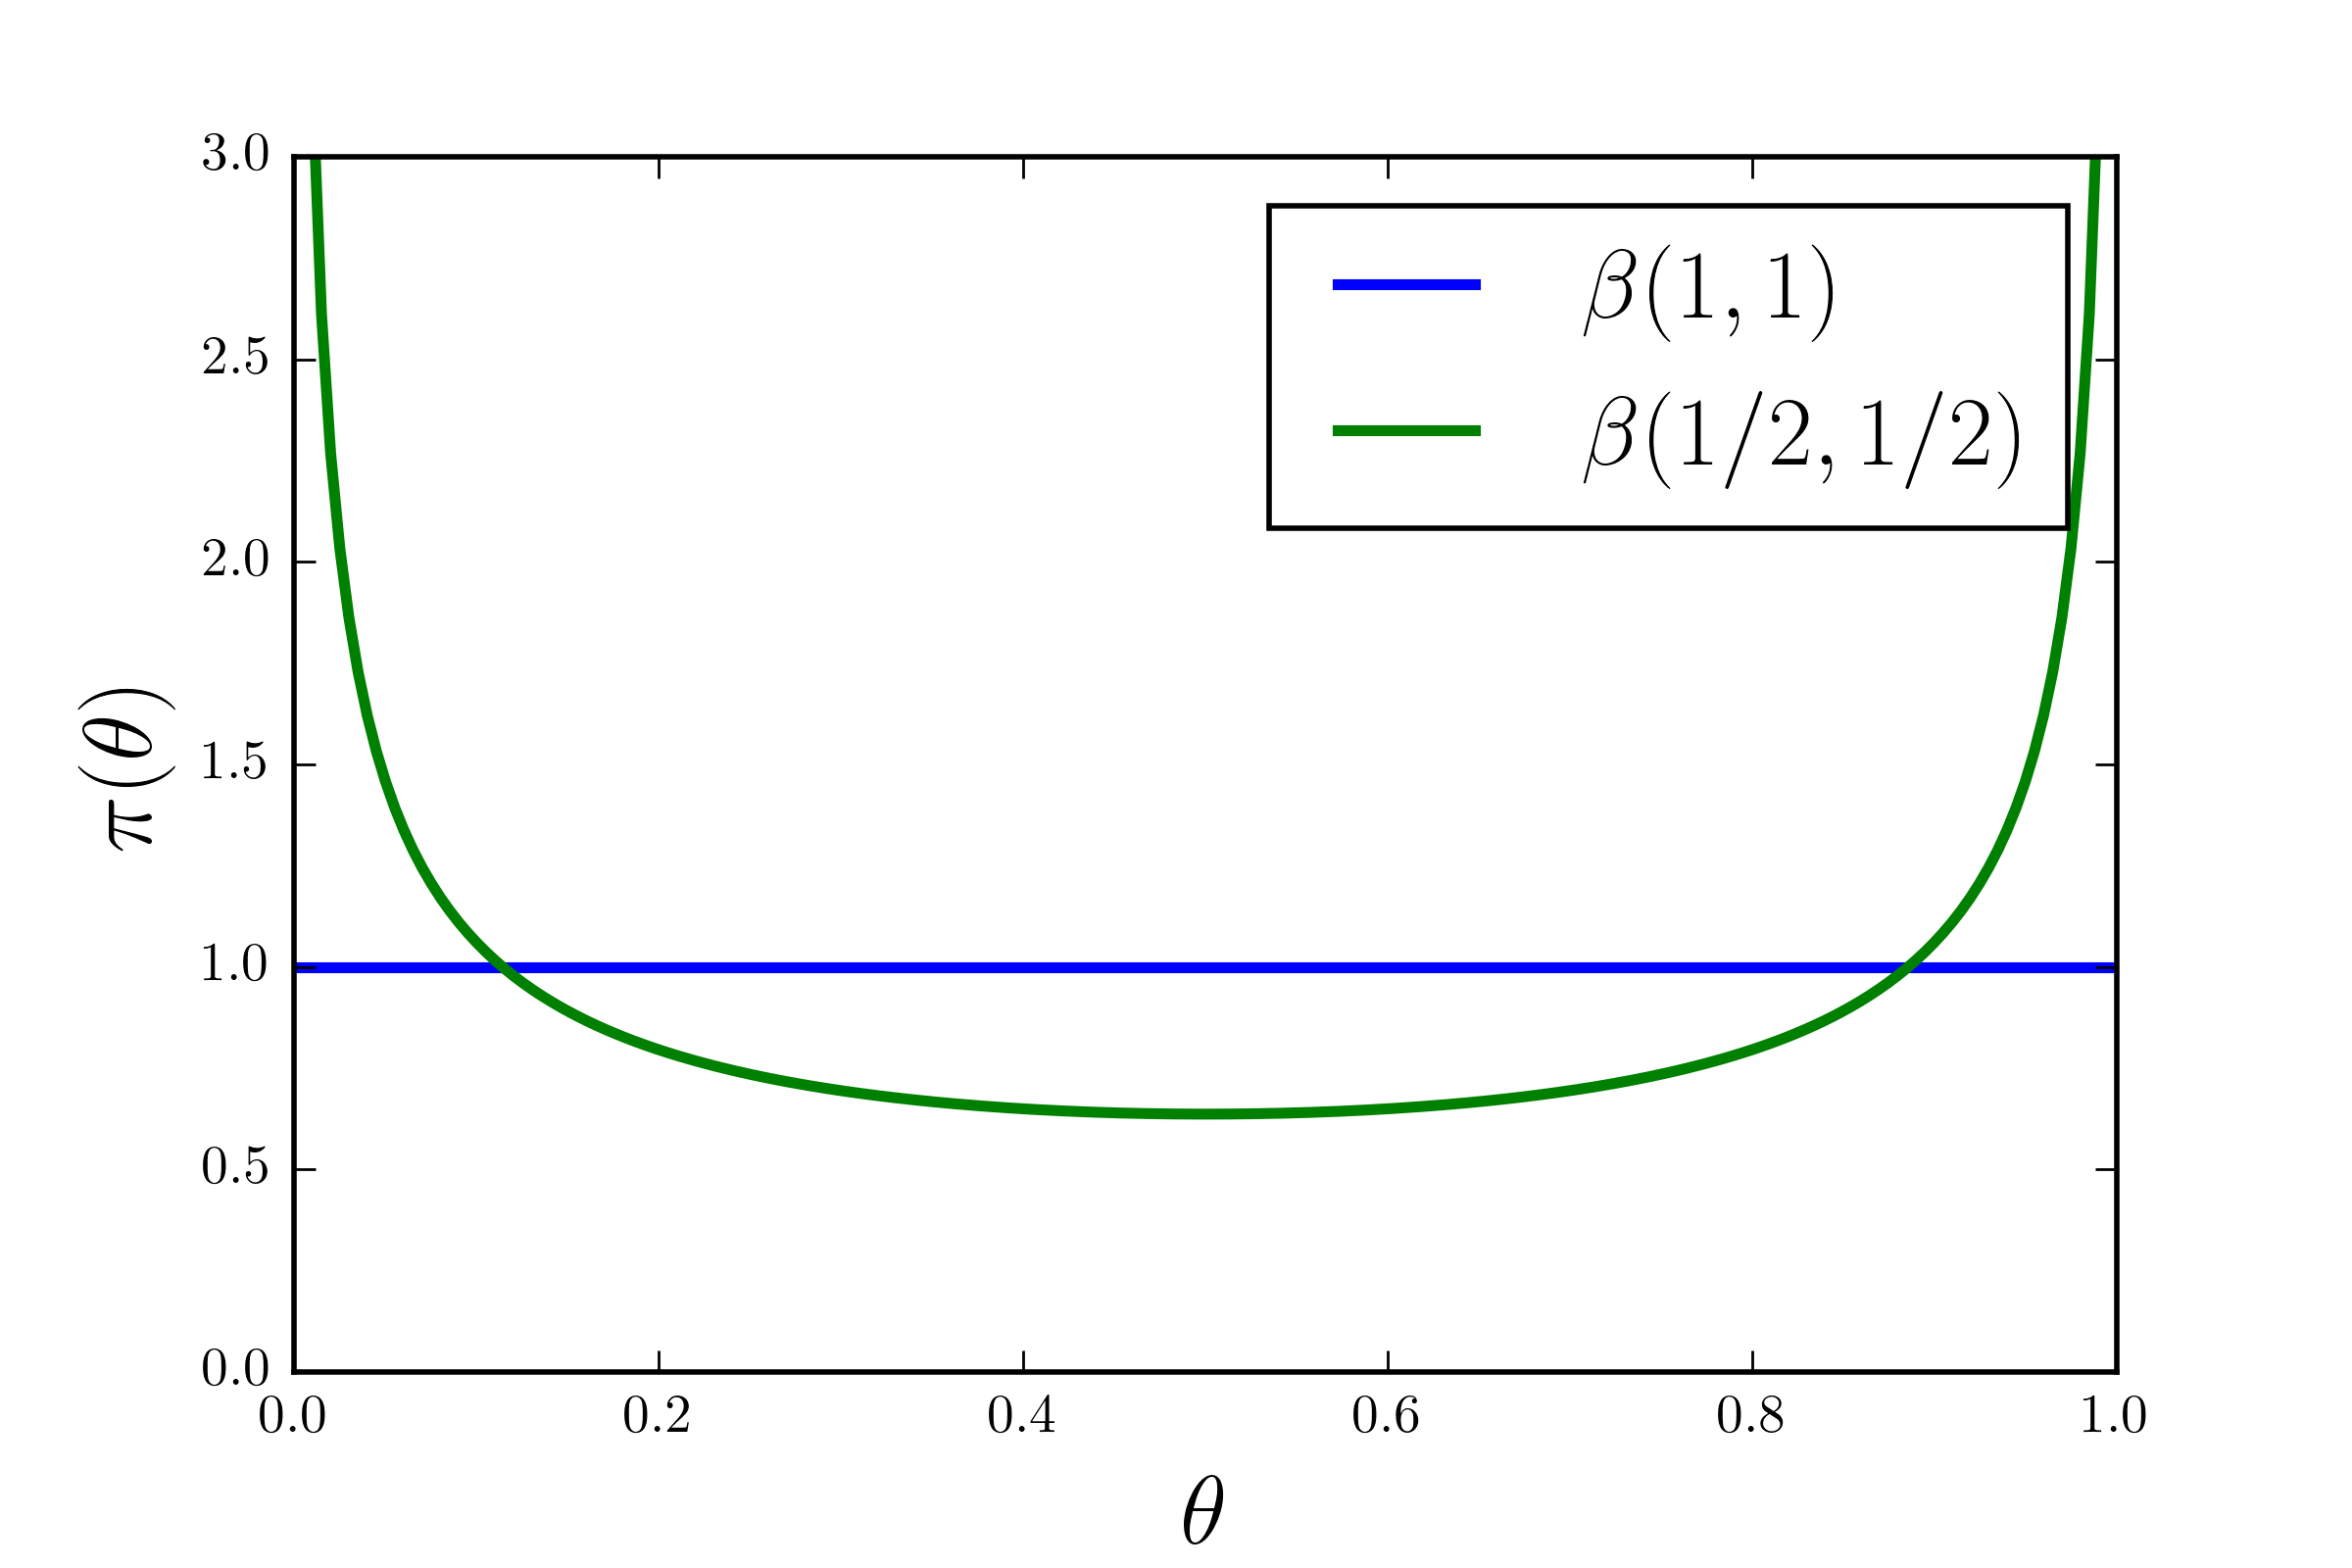
\includegraphics[width=0.5\textwidth]{figures/beta_comparison.png}
\caption{Сравнение равномерного априорного распределения $\beta(1, 1)$ и априорного распределения Джеффриса $\beta(\frac12, \frac12)$}
\label{fig:beta_comparison}
\end{figure}
\end{example}

\subsection{Связь сопряженного априорного распределения и априорного распределения Джеффриса}

Для примера с биномиальным распределением сопряженное априорное распределение и априорное распределение Джеффриса совпадают.
Для нормального распределения это не так: для математического ожидания $\pi_J(\mu) \sim 1$, а $\pi_J(\sigma) \sim \frac{1}{\sigma}$,
в то время сопряженное априорное распределение $\pi_C(\sigma)$ для $\sigma$ --- обратное гамма-распределение.

Однако, если для плотности обратного гамма-распределения с параметрами $a, b$:
\[
\pi_{a, b}(\sigma) \propto \frac1{\sigma^{-(a + 1)}} e^{\frac{-b}{\sigma}}
\]
устремить $a, b$ к нулю, то в пределе получим априорное распределение Джеффриса с плотностью, пропорциональной $\frac{1}{\sigma}$.
Параметры $a$ и $b$ априорного распределения можно интерпретировать как количество наблюдений и меру концентрации параметра в области.
Таким образом, устремляя эти два параметра к нулю, мы получаем априорное распределение, в котором нет <<наблюдений>> и параметр равномерно распределен по всему пространству.

Разумеется, модели в математической статистике не исчерпываются этими двумя примерами, и в общем случае сопряженное априорное распределение и априорное распределение Джеффриса могут быть никак не связаны.

\subsection{Ограничения априорного распределения Джеффриса}

Проблемы у такого подхода начинаются, когда размерность пространства параметров $\pD > 1$. 
По аналогии с одномерным случаем определим априорное распределение Джеффриса как 
\[
\pi_J(\vecT) = |I(\vecT)|^{\frac12}.
\]
Тогда по определению
\[
I(\vecT)_{ij} = -\bbE_{\vecT} \left[ \frac{\partial^2 \log p(X | \vecT)}{\partial \theta_i \partial \theta_j} \right].
\]

\begin{example}
Пусть мы наблюдаем вектор $\vecX$ из многомерного нормального распределения: 
\[
\vecX \sim \mathcal{N}(\vecT, I)
\]
для $\vecX \in \bbR^{\pD}$.
Задача состоит в оценке $\|\vecT\|^2$.

В таком случае априорное распределение Джеффриса будет равномерным.
Апостериорное распределение в таком случае будет нецентральным $\xi^2$ распределением с $\pD$ степенями свободы.
Апостериорное среднее
\[
\bbE (\|\vecT \|^2 | \vecX) = \|\vecX \|^2 + \pD.
\]

Получается, что, используя априорное распределение Джеффриса, мы получаем результат, смещенный в большую сторону на $\pD$,
в то время как обычно мы хотим получить в некотором роде регуляризирующую оценку.
Например, математическое ожидание классической вероятностной оценки будет $\|\vecX \|^2 - \pD$.

Так же будет происходить и в многомерном случае.
В силу того, что большая часть равномерного распределения находится на большом расстоянии от начала координат, 
Байесовские оценки часто будут смещены, причем в большую сторону.
\end{example}

Рассмотрим теперь двумерный пример.
\begin{example}
Пусть $x \sim \mathcal{N}(\mu, \sigma^2)$, и пусть $\vecT = (\mu, \sigma^2)^\T$.
Подсчитаем производные и получим информационную матрицу Фишера:
\begin{align*}
I(\vecT) &= -
\begin{pmatrix}
\frac{1}{\sigma^2}           & \frac{2 (x - \mu)}{\sigma^2} \\
\frac{2 (x - \mu)}{\sigma^2} & \frac{3}{\sigma^4} (x - \mu)^2 - \frac{1}{\sigma^2} \\
\end{pmatrix} = \\
&= 
\begin{pmatrix}
\frac{1}{\sigma^2} & 0 \\
0 & \frac{1}{\sigma^2} \\
\end{pmatrix},
\end{align*}
так как $\bbE_{\vecT} (x - \mu) = 0$, $\bbE_{\vecT} (x - \mu)^2 = \sigma^2$.
Следовательно, априорное распределение Джеффриса имеет вид:
\[
\pi_J(\vecT) = |I(\vecT)|^{\frac12} \propto \frac{1}{\sigma^2}.
\]
У такого априорного распределения ряд недостатков --- например, низкая скорость сходимости.
Сам Джеффрис предложил использовать априорное распределение $\pi_{J'}(\vecT) \propto \frac{1}{\sigma}$.
Такое априорное распределение лучше с точки зрения естественных предположений и позволяет получить оценки, статистические свойства которых лучше.
Оказывается, что $\pi_{J'}$ совпадает с опорным априорным распределением, про которое мы поговорим в следующей главе.
\end{example}

Получается, что у априорного распределение Джеффриса есть следующие недостатки:
\begin{itemize}
	\item Равномерность априорного распределения может в некоторых случаях приводить к неразумным с точки зрения здравого смысла оценкам.
	\item Непонятно, как правильно обобщить его на многомерный случай.
\end{itemize}

Чтобы решить эти проблемы, было предложено использовать опорное априорное распределение.
у него в меньшей степени проявляются недостатки перечисленные выше и, кроме того, оно позволяет посмотреть на задачу выбора неинформативного априорного распределения с точки зрения теории информации.